\documentclass[t]{beamer}
\usetheme[deutsch]{KIT}
\setbeamercovered{transparent}
\setbeamertemplate{navigation symbols}{}

\KITfoot{Tutoriumsmaterial von Joachim Priesner, Sebastian Ullrich und Max Wagner \hspace{2.5cm} Basierend auf den Folien von Simon Stroh und Moritz v. Looz}
\usepackage[utf8]{inputenc}
\usepackage{amsmath}
\usepackage{ifthen}
\usepackage{amssymb}
\usepackage{tikz}
\usepackage{ngerman}
\usetikzlibrary{automata}
\usenavigationsymbols


\title{Theoretische Grundlagen der Informatik}
\subtitle{Tutorium}
\author{Moritz von Looz, Simon Stroh}

\institute[ITI]{Institut für Theoretische Informatik}

\TitleImage[height=\titleimageht]{images/tmaschine.png}

\newcommand{\N}{\ensuremath{\mathbb{N}}}
\newcommand{\M}{\ensuremath{\mathcal{M}}}
\newcommand{\classP}{\ensuremath{\mathcal{P}}}
\newcommand{\classNP}{\ensuremath{\mathcal{NP}}}
\newcommand{\co}{\ensuremath{\mathsf{co\text{-}}}}
\newcommand{\pot}{\ensuremath{\mathcal{P}}}
\newcommand{\abs}[1]{\ensuremath{\left\vert #1 \right\vert}}
\newcommand{\menge}[2]{\ensuremath{\left\lbrace #1 \,\middle\vert\, #2 \right\rbrace}}
\newcommand{\ducttape}[1]{\vspace{#1}}
\newcommand{\neglit}[1]{\overline{#1\vphantom{x^a}}}
\newcommand{\recipe}{\raisebox{-.3cm}{
\includegraphics[scale=.15]{images/chefs-cap.png}}\hspace{0.2cm}}

\newcommand{\invincible}{\setbeamercovered{invisible}} %  "Yesss! I am invincible!!" (Boris Grishenko)
\newcommand{\vincible}{\setbeamercovered{transparent}}

% \@ifundefined{tikzset}{}{\tikzset{initial text=}} % Text "start" bei Startknoten unterdrücken
\tikzstyle{every node}=[thick]
\tikzstyle{every line}=[thick]

\newcommand{\tutnr}[1]{
  \subtitle{Tutorium #1}
	\begin{frame}
		\maketitle
	\end{frame}
}

\newcommand{\uebnr}[1]{
  \subtitle{Anmerkungen zum #1. Übungsblatt}
	\begin{frame}
		\maketitle
	\end{frame}
}

\begin{document}

\tutnr{3}
\section{Nerode-Relation}
\subsection{Nerode-Relation}
\begin{frame}
 \frametitle{Nerode-Relation}
 \begin{block}{Definition 2.25}
 Für eine Sprache \(L \subseteq \Sigma^*\) ist die \emph{Nerode-Relation} \(R_L\) definiert durch:
  
 Für alle $x, y \in \Sigma^*$ ist 
 \begin{center}$x$ $R_L$ $y$ $\Longleftrightarrow$ für alle $z \in \Sigma^*$ gilt $(xz \in L \Leftrightarrow yz \in L)$
 \end{center}

 \end{block}
  \begin{block}{Erinnerung}
   Die minimale Anzahl an Zuständen eines endlichen Automaten einer Sprache $L \subseteq \Sigma^*$ entspricht dem Index der Nerode-Relation.
  \end{block}
\end{frame}
\begin{frame}
\frametitle{Aufgabe zur Nerode-Relation}
Gib für die folgenden Sprachen jeweils die Äquivalenzklassen bezüglich der Nerode-Relation $R_L$ an. Welche der Sprachen sind regulär? Begründe deine Antwort. Konstruiere für diese Sprachen jeweils den Minimalautomaten.
\begin{itemize}
  \item $L_1 = \{a^{2i} \mid i \in \mathbb{N}_0, i \geq 1\}$, $\Sigma=\{a\}$
  \item $L_2 = \{ww \mid w \in \{0,1\}^*\}$, $\Sigma=\{0,1\}$
\end{itemize}
\end{frame}

\section{Turingmaschinen}
\subsection{Registermaschine}
\begin{frame}
\frametitle{Registermaschine}
Annähernd realistisches Rechnermodell. Bestehend aus:
 \begin{itemize}
  \item Befehlszähler (b)
  \item Akkumulator 
  \item Register (= Speicher)
  \item Programm
 \end{itemize}
Der Speicher der Registermaschine ist unendlich und eindeutig adressierbar.
\begin{figure}[H]
\begin{center}
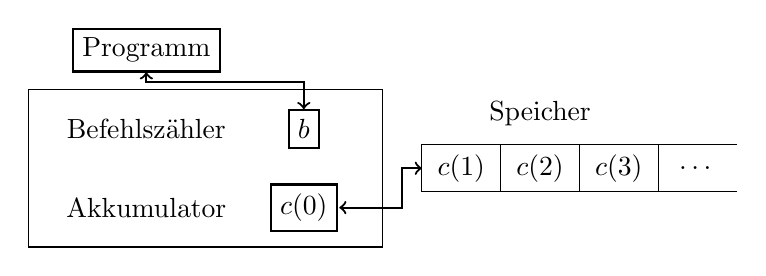
\begin{tikzpicture}
\node[draw] at (0,0) {Programm};
\node at (0,-1) {Befehlszähler};
\node[draw] at (2,-1) {$b$};
\node at (0,-2) {Akkumulator};
\node at (5,-0.8) {Speicher};
\node[draw] at (2,-2) {$c(0)$};
\draw (3.5,-1.8) rectangle (4.5,-1.2);
\node at (4,-1.5) {$c(1)$};
\draw (4.5,-1.8) rectangle (5.5,-1.2);
\node at (5,-1.5) {$c(2)$};
\draw (5.5,-1.8) rectangle (6.5,-1.2);
\node at (6,-1.5) {$c(3)$};
\draw (6.5,-1.8) -- (7.5,-1.8);
\node at (7,-1.5) {\ldots};
\draw (6.5,-1.2) -- (7.5,-1.2);
\draw (-1.5,-2.5) rectangle (3,-0.5);
\draw[<->,thick] (0,-0.28) -- (0,-0.4) -- (2,-0.4) -- (2,-0.75);
\draw[<->,thick] (2.45,-2) -- (3.25,-2) -- (3.25,-1.5) -- (3.5,-1.5);
\end{tikzpicture}
\end{center}
\end{figure}
\end{frame}

\subsection{Turingmaschine}
\begin{frame}
\frametitle{Turingmaschine}
Eine Registermaschine ist zwar physikalischen Rechnern ähnlich, aber unhandlich, um Beweise zu führen.
Daher ist ein abstrakteres Modell hilfreich. \\
$\rightarrow$ Turingmaschine
\pause
\begin{block}{Turingmaschine}
Die Turingmaschine besteht aus einem beidseitig \emph{unendlichen} Eingabe- und Rechenband
mit einem frei beweglichen Lese-/Schreibkopf, der von einer \emph{endlichen} Kontrolle gesteuert wird. 
\end{block}

\begin{center}
	\only<2->{\includegraphics[scale=0.5]{images/tmaschine.png}}
\end{center}
\end{frame}
\begin{frame}
\frametitle{Turingmaschine}
\begin{block}{Definiton}
Eine Turingmaschine wird definiert als ein 7-Tupel bestehend aus:
 \begin{itemize}
 \item $Q$, einer endlichen Zustandsmenge
 \item $\Sigma$, einem endlichen Eingabealphabet
 \item $\sqcup$, einem Blanksymbol mit $\sqcup \notin \Sigma$
 \item $\Gamma$, einem endlichen Bandalphabet mit $\Sigma \cup\{\sqcup\} \subseteq \Gamma$
 \item $s \in Q$, einem Startzustand
 \item $\delta$, einer Übergangsfunktion $\delta: Q\times\Gamma \rightarrow Q\times\Gamma\times\{L, R, N\}$
 \item $F \subseteq Q$, einer Menge an Endzuständen
 \end{itemize}
\end{block}
\begin{block}{Bemerkung}
 Für $q\in F$ gilt: $\forall a \in \Gamma: \delta(q, a) = (q, a, N)$, d.h. die Berechnung der Turingmaschine stoppt.
\end{block}
\end{frame}

\frame{
	\frametitle{Graph einer Turingmaschine}
	\begin{center}
	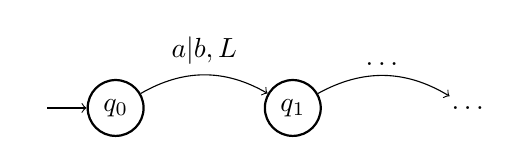
\begin{tikzpicture}[node distance=2.25cm,auto]
	\node(q0)[draw,circle,thick]{$q_0$};
	\node (s) [node distance=1cm,left of =q0]{};
	\node(q1)[draw,circle,thick,right of=q0]{$q_1$};
	\node(qx)[right of=q1]{\dots};

	\path[->]       (s) edge (q0)
	                (q0) edge[bend left] node{$a|b,L$} (q1)
			                (q1) edge[bend left] node{\dots} (qx);
					\end{tikzpicture}
					\end{center}

					Dabei steht die Kantenbeschriftung "`$a|b,L$"' für den Übergang $\delta(q_0,a) =
					(q_1,b,L)$.

					\vspace{2mm}
					Falls es für einen gegebenen Zustand und ein gegebenes
					Symbol keinen Zustandsübergang gibt, bricht die Maschine die Berechnung ab. 
}

\begin{frame}
	\frametitle{Turingmaschine: Beispiel}
	
	Seien $\Sigma = \{0,1\}$, $\Gamma = \{0,1,\sqcup\}$ und die Turingmaschine $\M =(\{q_0, q_1,q_2,q_f\},\Sigma, \sqcup, \Gamma,\delta,q_0,\{q_f\})$ mit folgender Überführungsfunktion gegeben:
	
	\begin{center}
	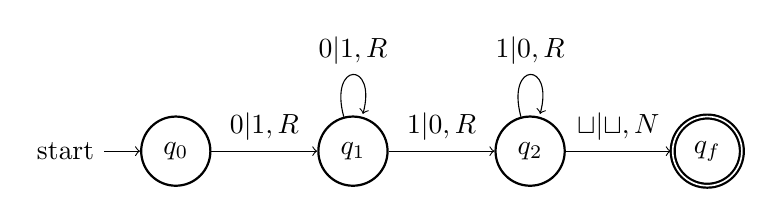
\begin{tikzpicture}[node distance=2.25cm,auto]
	\node(q0)[state,initial]{$q_0$};
	\node(q1)[state,right of=q0]{$q_1$};	
	\node(q2)[state,right of=q1]{$q_2$};	
	\node(qf)[state,accepting,right of=q2]{$q_f$};	

	\path[->]       (q0) edge node{$0|1,R$} (q1)
					(q1) edge node{$1|0,R$} (q2)
	                (q1) edge[loop above] node{$0|1,R$} (q1)	                
			        (q2) edge[loop above] node{$1|0,R$} (q2)
			        (q2) edge node{$\sqcup|\sqcup,N$} (qf);
					\end{tikzpicture}
					\end{center} 
					
	\begin{itemize}
		\item Welche Wörter akzeptiert \M{}?
		\item Wie verändert \M{} die Eingabe?
	\end{itemize}			
\end{frame}


\begin{frame}
\frametitle{Konfigurationen}
Sei $\mathcal{M} =(Q,\Sigma, \sqcup, \Gamma,\delta,s,F)$ eine Turingmaschine.

Angabe des aktuellen Berechnungszustandes: \emph{Konfiguration}

$$w(q)av$$ 

wobei $w,v \in \Gamma^*, a \in \Gamma$ und $q\in Q$. \\

Dies bedeutet:

\begin{itemize}
	\item $\mathcal{M}$ befindet sich im Zustand $q$.
	\item Der Lesekopf steht auf dem Zeichen $a$.
	\item Links vom Lesekopf steht das Wort $w$ und rechts davon das Wort $v$ auf dem Rechenband.
\end{itemize}
\end{frame}

\subsection{Aufgaben}

\begin{frame}
\frametitle{Aufgabe: Turingmaschine}
\vspace{-1cm}
\begin{center}
     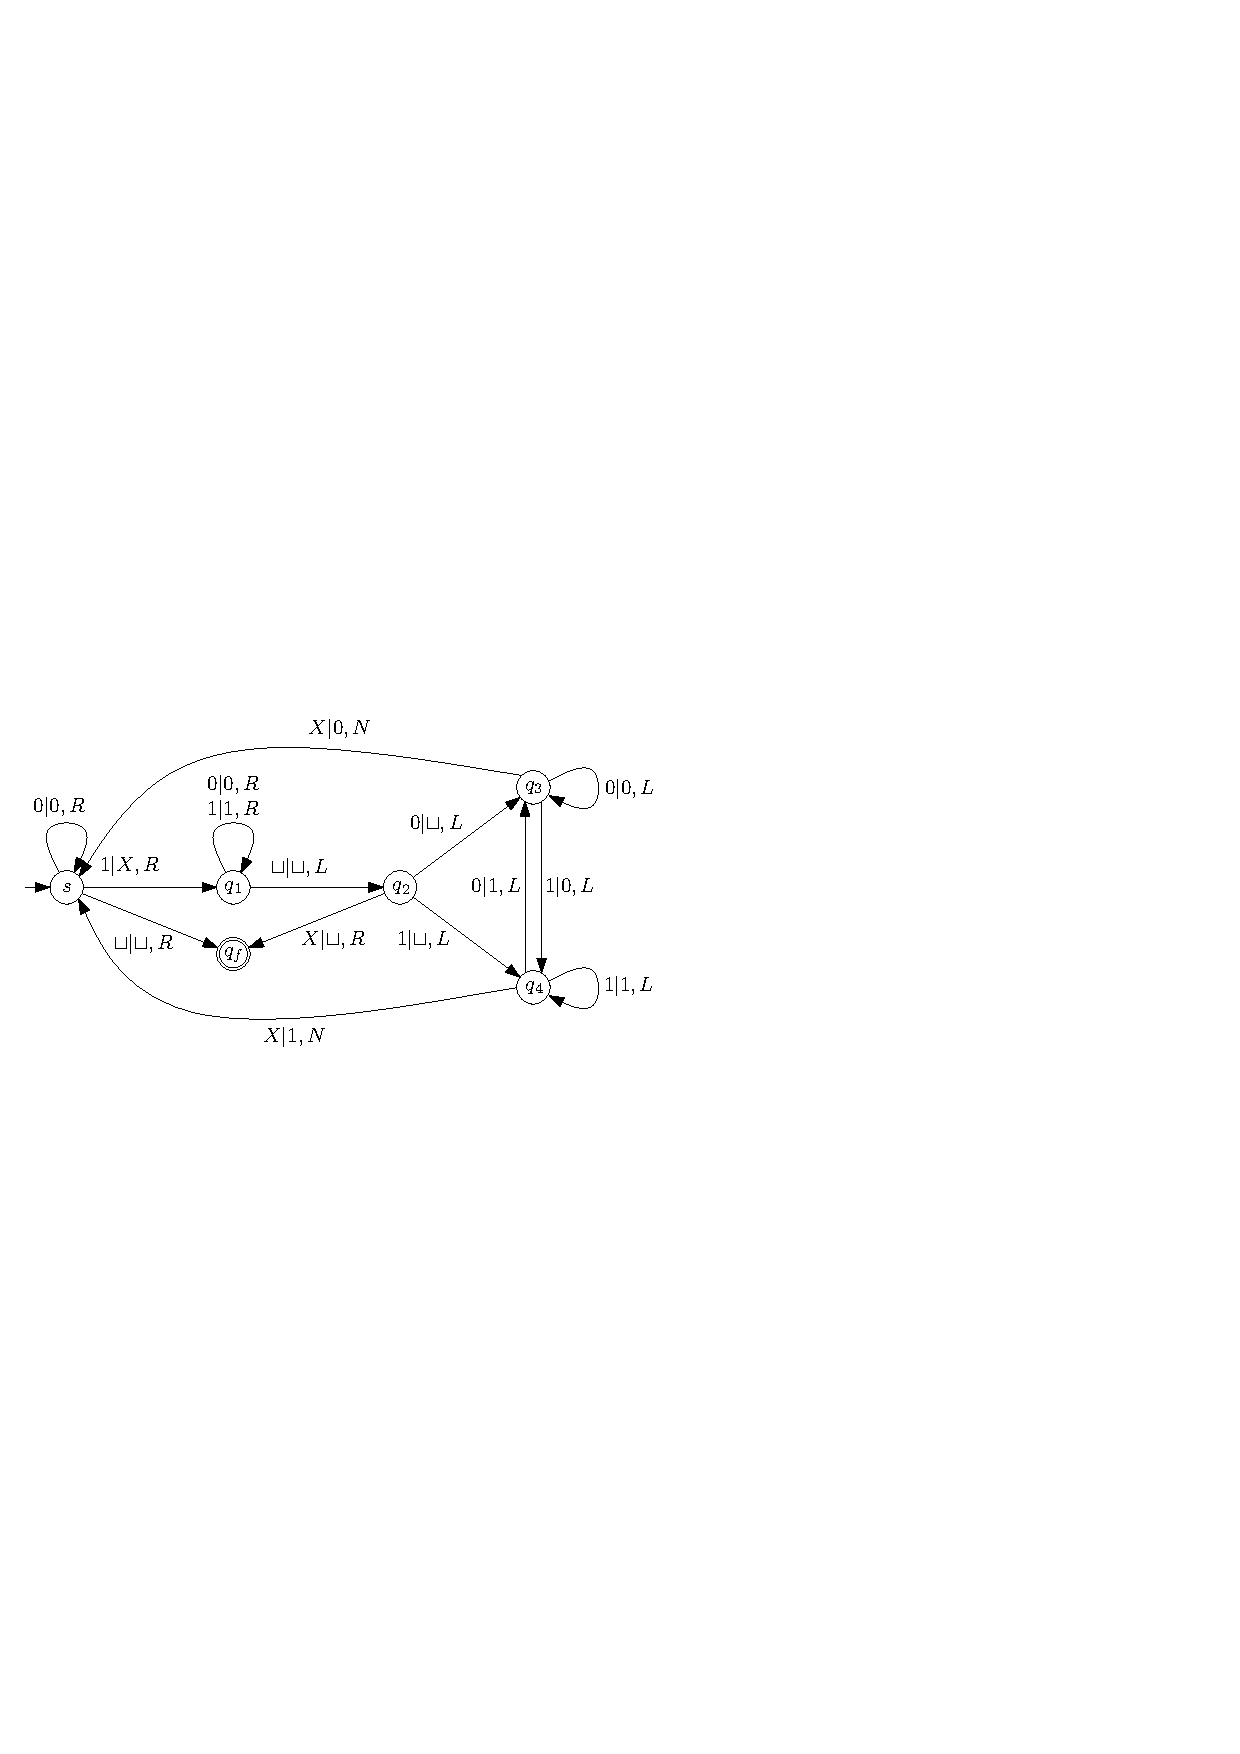
\includegraphics[scale=0.7]{images/Uebungsblatt_2_A5}
   \end{center}
   
\begin{enumerate}
 \item Welche Konfigurationen durchläuft die Maschine bei Eingabe des
  Wortes $01010$?

 \item Welche Aufgabe haben die Zustände $q_2, q_3$ und $q_4$? 
       (Hinweis: Überlege dir dazu, was passiert, wenn $\mathcal{M}$ sich im Zustand $q_2$ befindet und der Lesekopf auf dem letzten Zeichen der Eingabe steht, bis zu dem Zeitpunkt, zu dem das erste Mal $X$ gelesen wird.)  

 \item Wie verändert $\mathcal{M}$ die Eingabe?

\end{enumerate}
\end{frame}

\begin{frame}
\frametitle{Aufgabe: Turingmaschine}
Entwirf eine deterministische Turing-Maschine $\mathcal M := (Q, \Sigma, \Gamma, \delta, s, F)$, die genau die folgende Sprache akzeptiert: $$L:=\menge{ww^R}{ w \in \{a, b\}^*}$$ wobei $w^R$ das "`Spiegelwort"'~zu $w$ ist.
Dies ist die Sprache der Palindrome gerader Länge.

\begin{enumerate}
	\item Beschreibe kurz in Worten, wie deine Turing-Maschine arbeitet.
	\item Spezifiziere $\mathcal M$ explizit durch Angabe eines Zustandsdiagramms oder einer formalen Spezifikation.
\end{enumerate}
\end{frame}
\begin{frame}
\frametitle{Aufgabe: Turingmaschine}
 \label{sec:busy_beaver}

Entwirf eine Turingmaschine, die aus drei Zuständen (plus einem
weiteren Haltezustand $q_f$) besteht und folgendes Verhalten hat:
\begin{quote}
  Angesetzt auf ein leeres Band schreibt sie möglichst viele ${\tt 1}$
  hintereinander und \textbf{hält} nach endlich vielen Schritten.
\end{quote}
Die Turingmaschine soll folgende Alphabete verwenden: $\Sigma = \{{\tt 1}\},
\Gamma = \Sigma \cup \{{\tt 0}\}$.  Insbesondere ist also ${\tt 0}$ das
Blanksymbol.

\begin{enumerate}
	\item Welche Konfigurationen durchläuft die Maschine, wenn sie auf dem leeren Band gestartet wird?
	\item Welche Konfigurationen durchläuft die Maschine bei Eingabe
des Wortes {\tt 101}?
\end{enumerate}
\end{frame}

\section{Schluss}
\subsection{Schluss}

\begin{frame}
\frametitle{Bis zum nächsten Mal!}
\begin{center}
  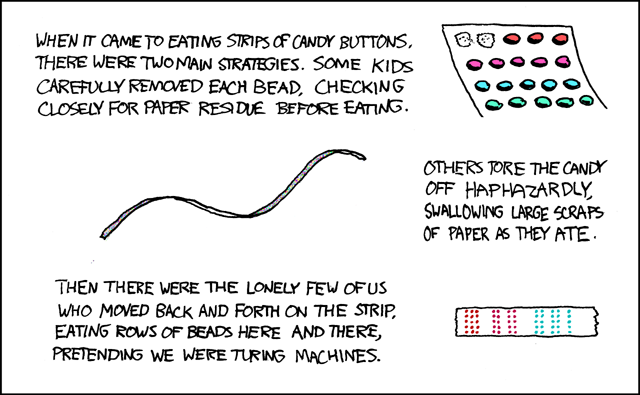
\includegraphics[height=0.8 \textheight]{images/xkcd_205.png} 
\end{center}

\begin{quote}\tiny{Nonrewritable tape?}
\end{quote}
\end{frame}

\frame{
  \frametitle{Lizenzen}
  \center
  \includegraphics[width=2em]{images/by}
  \includegraphics[width=2em]{images/cc}
  \includegraphics[width=2em]{images/sa}
  \\
  {\tiny

Dieses Werk ist unter einem ``Creative Commons Namensnennung-Weitergabe unter gleichen Bedingungen 3.0 Deutschland``-Lizenzvertrag lizenziert. Um eine Kopie der Lizenz zu erhalten, gehen Sie bitte zu \href{http://creativecommons.org/licenses/by-sa/3.0/de/}{http://creativecommons.org/licenses/by-sa/3.0/de/} oder schreiben Sie an Creative Commons, 171 Second Street, Suite 300, San Francisco, California 94105, USA.\\
  \vspace{1cm}
  Davon ausgenommen sind das Titelbild, welches aus der März-April 2002 Ausgabe von American Scientist erschienen ist und ohne Erlaubnis verwendet wird, sowie das KIT Beamer Theme. Hierfür gelten die Bestimmungen der jeweiligen Urheber.
  \vspace{1cm}
  \\ 
  }
  %Habe hier die Reihenfolge etwas umgestellt, weil die Formatierung bei mir komisch aussah. 
  %Wenn es bei dir anders ist, kannst du es auch wieder zurückändern, dann haben wir unterschiedliche Kompilieroptionen
}

\end{document}
